% =====================================================================
%  report.tex -- final report, DML 2026 (IEEEtran, max 4 pages incl. refs)
%  Evidence levels are kept apart in the text: "on the test set" =
%  pre-registered confirmatory pass; "on validation" = exploratory.
%  Sources of every number: docs/lab-notebook.md and docs/results/*.
%  Figures: img/fig_block.pdf (Fig. 1, the poster's TikZ figure) and
%  img/fig_results.pdf (Fig. 2, matplotlib at column width from the
%  numbers of Tab. I; docs/report/make_fig_results.py).
% =====================================================================
\documentclass[conference]{IEEEtran}
\IEEEoverridecommandlockouts
\usepackage{cite}
\usepackage{amsmath,amssymb}
\usepackage{graphicx}
\usepackage{booktabs}
\usepackage{xcolor}
\usepackage{url}
\usepackage{float}

% ---- names of the configurations (paper name  <-  code name) --------
\newcommand{\B}{B}                                  % B (DfpNet, 2.33M)
\newcommand{\Blarge}{B-large}                       % B-large (33 base ch.)
\newcommand{\Msh}[1]{M$^{\mathrm{sh}}_{#1}$}        % MD<l>: shared-weight SS2D
\newcommand{\M}[1]{M$_{#1}$}                        % MDv<l>: SS2D as in VMamba
\newcommand{\Mloc}{M$^{\mathrm{loc}}_{64}$}         % MDv64-local: scan removed (FINAL)
\newcommand{\Mdec}{M$^{\mathrm{dec}}_{64}$}         % MDv64-dec: same block in the decoder
\newcommand{\SA}[1]{SA$_{#1}$}                      % SA<l>: self-attention block
\newcommand{\Conv}{Conv$_{64}$}                     % Conv64: plain residual conv block
\newcommand{\DR}{DR-M}                              % DRv11: deep path -> 11 SS2D blocks at 8x8
\newcommand{\TR}{TR}                                % TR: truncated net, no deep path
\newcommand{\relvy}{$\mathrm{rel}_{v_y}$}
\newcommand{\relall}{$\mathrm{rel}_{\mathrm{all}}$}
\newcommand{\relp}{$\mathrm{rel}_{p}$}
\newcommand{\ci}[2]{[$#1$,\,$#2$]}                  % 95% interval

\begin{document}

\title{Airfoil Flow Prediction: \textit{Where} and \textit{Why} Mamba Blocks Enhance U-Net Architectures}

\author{\IEEEauthorblockN{Cristiano Corona, Francesca Marina Pozzi}
\IEEEauthorblockA{Deep Machine Learning, Group 62\\
\textit{Chalmers University of Technology}}
}
\maketitle

\begin{abstract}
A convolutional U-Net (DfpNet, Thuerey et al.~\cite{thuerey2020}) approximates
the solution of the Reynolds-averaged Navier--Stokes (RANS) equations around
airfoils in a single forward pass, far more efficiently than a numerical solver.
Since convolutions are local, whereas the pressure obeys a Poisson equation whose
elliptic operator couples the whole domain, we investigate whether a Mamba block, a
selective state-space model with cost linear in the number of tokens, improves
this network, where it should be placed, and how it compares with
self-attention. At the deepest levels it adds nothing, although stacked Mamba
blocks can replace the deep convolutional path without a measurable loss. At
the highest resolution ($\boldsymbol{64\times64}$) it reduces the relative error on $\boldsymbol{v_y}$ by
18\% on unseen airfoils in a pre-registered test; self-attention gives a
comparable gain at about 17 times the training cost. Ablations show that most
of the gain persists without the SSM, the core of Mamba (a $\boldsymbol{13\%}$ reduction, also
confirmed on the test set), in line with MambaOut~\cite{yu2025mambaout}. With
8 times more training data, the gain halves but persists near the airfoil.
\end{abstract}

\begin{IEEEkeywords}
RANS, U-Net, Mamba, SSMs, ablation.
\end{IEEEkeywords}

% =====================================================================
\section{Introduction}

Computational fluid dynamics (CFD) predicts fluid flows by solving their
governing equations numerically: for a Newtonian fluid, the Navier--Stokes
(NS) equations are used. However, at high Reynolds numbers
$\mathrm{Re}=Uc/\nu$ (flow speed $U$, chord $c$, kinematic viscosity $\nu$),
direct numerical simulation of turbulent flows is prohibitive, and the
Reynolds-averaged Navier--Stokes (RANS) equations are solved instead to model
the mean flow affordably.

A neural network trained on RANS solutions can replace the numerical solver when a design loop requires thousands of solutions, mapping geometry and flow conditions to the solution in a single forward pass. Thuerey et al.~\cite{thuerey2020} showed
that a convolutional U-Net, DfpNet, predicts pressure and velocity around
airfoils with a combined relative error (Sec.~\ref{sec:metrics}) below 3\%. While convolutions operate locally, requiring a U-Net to repeatedly reduce resolution to span the entire domain, pressure is governed by an elliptic Poisson equation, making its local values globally dependent on the entire flow field. Global mixing
mechanisms can overcome this mismatch: self-attention~\cite{vaswani2017} relates all pairs of tokens at quadratic cost, while Mamba~\cite{gu2024mamba}, a selective state-space model (SSM), propagates information at linear cost, and VMamba~\cite{liu2024vmamba} extends it to images.

We ask whether a Mamba block improves DfpNet, where in the network it helps,
and which of its components is responsible: we insert one residual block at
one resolution at a time, then remove parts of it, and confirm the main
findings with pre-registered tests on unseen airfoils.\footnote{Code, results and lab notebook:
\url{https://github.com/CristianoCorona/MambaDeepFlow}.}

% =====================================================================
\section{Background}
\label{sec:background}

\subsection{Reynolds-averaged Navier--Stokes equations}
\label{sec:rans}

For turbulent flows at high Reynolds number ($\mathrm{Re}\in[0.5,5]\times10^6$
in our data), the RANS approach decomposes velocity and pressure into a mean and a
fluctuating part, $u_i=\bar u_i+u_i'$ and $p=\bar p+p'$, with
$\overline{u_i'}=0$; the smoother mean fields can thus be computed on much coarser grids. For a steady, incompressible flow, averaging the continuity and momentum equations yields equations for $\bar u_i$ and $\bar p$ in which the nonlinear convective term produces the Reynolds stresses $\overline{u_i'u_j'}$, new unknowns that leave the system unclosed. In the
training data~\cite{thuerey2020}, the system is completed with the Boussinesq hypothesis, which expresses the stresses through a turbulent viscosity, obtained from the one-equation Spalart--Allmaras model~\cite{spalart1992}. Taking the divergence of the averaged momentum equation and using continuity ($\partial_i\bar u_i=0$), the mean pressure satisfies a Poisson equation ($\rho$: density; repeated indices summed)
\begin{equation}
  \nabla^2 \bar p = -\rho\,\partial_i\partial_j
    \big(\bar u_i\bar u_j + \overline{u_i'u_j'}\big),
  \label{eq:poisson}
\end{equation}
which is elliptic: the pressure at any point depends on the source over the
whole domain (\emph{global coupling}). The mean fields $\bar p$, $\bar u_x$,
$\bar u_y$ are the targets of the network, denoted  by $p$, $v_x$, $v_y$ below.

\subsection{U-Net and receptive field}
\label{sec:unet}

A U-Net~\cite{ronneberger2015} uses skip connections to concatenate feature
maps from the encoder to the decoder. DfpNet~\cite{thuerey2020}
(Fig.~\ref{fig:arch}, top) is symmetric, employs seven stride-2 convolutions
($128\times128$ to $1\times1$, 32 to 256 channels, 2.33\,M parameters), and
is trained with an L1 loss. Its first layer is a single convolution, so the
$64\times64$ skip features undergo minimal processing; the receptive field
grows with depth, from 4\,px at $64\times64$ to 46\,px at $8\times8$, while
the deeper stages (79\% of the weights) extend it to the whole domain. Thus,
the U-Net already covers the whole domain, but does little processing at high
resolution.

%A U-Net~\cite{ronneberger2015} uses skip connections to concatenate feature maps from the encoder to the decoder. In particular, DfpNet~\cite{thuerey2020} is symmetric, and its encoder employs seven stride-2 convolutions to reduce spatial dimensions from $128\times128$ down to $1\times1$ while increasing channel depth from 32 to 256. With 2.33 M parameters, the network is trained using an L1 loss. Its first layer comprises a single convolution, meaning the $64\times64$ features passed to the decoder via the skip connection undergo minimal processing; receptive field expansion relies instead on network depth. Specifically, the receptive field grows from 4\,px at a resolution of $64\times64$ to 46\,px at $8\times8$, while the deeper stages below (accounting for roughly 79\% of the model's weights) extend it across the entire domain. Thus, while the U-Net already achieves global coverage, it lacks adequate representation capacity at high spatial resolutions.

\subsection{Global mixing: attention and selective state-space models}
\label{sec:mixing}

For global mixing, a feature map at spatial resolution $H \times W$ is reshaped into a sequence of $L = HW$ tokens $X \in \mathbb{R}^{L \times d}$. Self-attention~\cite{vaswani2017} evaluates all pairwise relationships via
\begin{equation}
  \mathrm{Attn}(X) = \mathrm{softmax}\left(QK^{\top}/\sqrt{d}\right)V,
  \label{eq:attn}
\end{equation}
where $Q$, $K$, $V$ are linear projections of $X$: all locations interact
directly, at cost $\mathcal{O}(L^2)$ ($1.7 \times 10^7$ pairs at $64 \times 64$).

Conversely, a state-space model (SSM) maps an input sequence $x(t)$ to an
output $y(t)$ through a hidden state $h(t)$, via $h'(t) = A h(t) + B x(t)$,
$y(t) = C h(t) + D x(t)$. Discretized with a step size $\Delta$ using a zero-order hold assumption ($\bar{A} = \exp(\Delta A)$, $\bar{B} \approx \Delta B$), it
reduces to the linear recurrence~\cite{gu2022s4}
\begin{equation}
  \mathbf{h}_t = \bar{A}\mathbf{h}_{t-1} + \bar{B}\mathbf{x}_t, \qquad \mathbf{y}_t = C\mathbf{h}_t + D\mathbf{x}_t,
  \label{eq:ssm}
\end{equation}
where $D$ is a per-channel skip term; each token influences all later ones at
a linear cost $\mathcal{O}(L)$. Mamba~\cite{gu2024mamba} makes the SSM
\emph{selective}: $\Delta$, $B$ and $C$ are computed from $\mathbf{x}_t$, so
each token controls how much of the state is kept; since the recursion can be written using an associative operator, it is computed by a hardware-aware parallel scan rather than
token by token.

VMamba~\cite{liu2024vmamba} brings this to images with the SS2D block
(Fig.~\ref{fig:arch}, bottom). An input projection expands the $n_c$ channels
into two branches of width $E$; one passes through a $3\times3$ depthwise
convolution and SiLU, is flattened in four orders (rows and columns, forward
and backward) and scanned by four SSMs with separate parameters; their outputs
are mapped back to 2-D, summed, normalised by a LayerNorm and gated by the
SiLU of the other branch, before an output projection back to $n_c$ channels.
MambaOut~\cite{yu2025mambaout} found
that the same block without the SSM (a Gated CNN) suffices for ImageNet
classification, but falls short of visual Mamba models on detection and
segmentation.

\subsection{Related work}

Attention~\cite{li2023hydrofoil,zhou2023tnn} and Mamba
blocks~\cite{cheng2024mno,zhang2026aeromamba} have been applied to flow
prediction, and to U-Nets~\cite{ma2024umamba}; these works report the gain of
the complete model, while we ask where the block helps and which part is
responsible.

% =====================================================================
\section{Method}

\subsection{Data, splits and pipeline}
\label{sec:data}

We adopt the dataset from~\cite{thuerey2020}, comprising UIUC airfoils
simulated via OpenFOAM at angles of attack up to $\approx 22.5^\circ$ on a
$128\times128$ grid. Network inputs include the two freestream velocity
components and the binary airfoil mask, while targets ($p$, $v_x$, $v_y$) are
normalized using $|\mathbf{v}_\infty|^2$ or $|\mathbf{v}_\infty|$ alongside
fixed maximum values. We train on the reduced set (6,400 samples across 1,456
airfoils) and evaluate on the official test set (90 samples, 30 unseen
airfoils). In the repository's default validation split, 390 of the 400 files
share airfoils with the training set, thus measuring unseen flow conditions on
known geometries. To validate on unseen shapes, we re-split strictly by
airfoil (5,998 training / 402 validation files across 1,371 / 85 airfoils):
the validation \relall{} of \B{} increases by $1.31\times$ and gets closer to
the test level (test/validation ratio 1.14, vs.\ 1.50 with the random split).
For \DR{} and \TR{} ($^{\dagger}$ in Table~\ref{tab:main}), 400 more files, one
per training airfoil, were held out as a seen-shape validation: they train on
5,598 files and are compared with \B{} retrained on the same split.

\subsection{Metrics and composition of the error}
\label{sec:metrics}

As in the official repository, the relative error of sample $s$ and channel
$c \in \{p, v_x, v_y\}$ is $\mathrm{rel}_c(s) = \sum_i|o_{c,i}-t_{c,i}| /
\sum_i|t_{c,i}|$, where $o$ and $t$ are prediction and target and $i$ runs over
the $128\times128$ cells; it is averaged over samples, in percent. \relall{}
pools all channels, which makes it a weighted mean:
\begin{equation}
  \mathrm{rel}_{\mathrm{all}}(s) = \sum_c w_c(s)\,\mathrm{rel}_c(s), \quad
  w_c(s) = \frac{\sum_i|t_{c,i}|}{\sum_{c'}\sum_i|t_{c',i}|}.
  \label{eq:relall}
\end{equation}
Validation weights average $0.046$ ($p$), $0.825$ ($v_x$) and $0.129$
($v_y$): $v_x$ is mostly free stream, so $\mathrm{rel}_{\mathrm{all}} \approx
\mathrm{rel}_{v_x}$, and one point gained on $v_y$ moves \relall{} by only
0.13. Since a mean of ratios is
dominated by samples with a small target signal (e.g.\ $v_y$ and $p$ at
low angles), we also report the aggregate ratio over all samples and the
median sample, plus the $v_y$ error in a 4-pixel wall band.

\begin{table*}[t]
\centering
\caption{Configurations and results. $\Delta$: mean over samples of the
seed-averaged difference to \B{} (test \relall{} $2.78\%$, test \relvy{}
$6.64\%$, val.\ \relvy{} $6.07\%$), in points, with 95\% two-level bootstrap
intervals (Sec.~\ref{sec:protocol}). Bold: confirmed pre-registered
hypotheses. Time: relative to \B. $^{\dagger}$Trained on 5,598 files
(Sec.~\ref{sec:data}), vs.\ \B{} on the same split (test \relall{} $2.90\%$); $^{\ddagger}$validation
only.}
\label{tab:main}
\footnotesize
\setlength{\tabcolsep}{3.1pt}
\begin{tabular}{@{}llrrcccc@{}}
\toprule
 & Block (position) & $\Delta$params & Time & Seeds & Val.\ $\Delta$\relvy & Test $\Delta$\relall & Test $\Delta$\relvy \\
\midrule
\Msh{8}  & shared-weight SS2D (enc.\ 8$\times$8) & +116,736 & 1.2$\times$ & 8 & $-0.24$ \ci{-0.46}{-0.04} & $+0.16$ \ci{-0.10}{+0.53} & $-0.04$ \ci{-0.59}{+0.49} \\
\M{8}    & SS2D (enc.\ 8$\times$8)                & +169,216 & 1.2$\times$ & 8 & $-0.09$ \ci{-0.35}{+0.16} & $-0.01$ \ci{-0.34}{+0.26} & $+0.00$ \ci{-0.52}{+0.50} \\
\Blarge  & none, 33 base channels                 & +147,720 & 1.3$\times$ & 8 & $-0.00$ \ci{-0.20}{+0.17} & -- & -- \\
\DR$^{\dagger}$ & deep path $\to$ 11 SS2D at 8$\times$8 & +22,656 & 2.9$\times$ & 5 & $-0.37$ \ci{-0.86}{+0.14} & $-0.12$ \ci{-0.51}{+0.29} & $-0.69$ \ci{-2.12}{+0.24} \\
\TR$^{\dagger}$ & deep path removed               & $-$1,838,720 & 0.8$\times$ & 5 & -- & $+0.57$ \ci{-0.01}{+1.03} & -- \\
\midrule
\M{64}   & SS2D (enc.\ 64$\times$64)              & +20,800 & 3.7$\times$ & 8 & $-0.75$ \ci{-1.03}{-0.50} & $-0.17$ \ci{-0.46}{+0.07} & $\mathbf{-1.17}$ \ci{-2.47}{-0.43} \\
\Mloc    & SS2D without scan (enc.\ 64$\times$64) & +7,232 & 1.6$\times$ & 8 & $-0.67$ \ci{-0.98}{-0.37} & $-0.12$ \ci{-0.35}{+0.15} & $\mathbf{-0.87}$ \ci{-1.60}{-0.35} \\
\midrule
\SA{64}$^{\ddagger}$  & self-attention (enc.\ 64$\times$64)   & +4,288 & 17$\times$ & 5 & $-0.61$ \ci{-0.86}{-0.39} & -- & -- \\
\Conv$^{\ddagger}$    & two 3$\times$3 convs (enc.\ 64$\times$64) & +6,956 & 1.2$\times$ & 5 & $-0.12$ \ci{-0.32}{+0.07} & -- & -- \\
\Mdec$^{\ddagger}$    & SS2D (dec.\ 64$\times$64)              & +20,800 & 3.7$\times$ & 5 & $-0.30$ \ci{-0.53}{-0.10} & -- & -- \\
\M{16}$^{\ddagger}$   & SS2D (enc.\ 16$\times$16)              & +55,936 & 1.3$\times$ & 5 & $-0.18$ \ci{-0.42}{+0.05} & -- & -- \\
5 variants$^{\ddagger}$ & \Mloc{} minus one ingredient       & 3.6k--43.5k & 1.3--1.6$\times$ & 5 & $-0.59$ to $-0.75$, all $<0$ & -- & -- \\
\bottomrule
\end{tabular}
\end{table*}

\subsection{Configurations}
\label{sec:configs}

\begin{figure}[t]
\centering
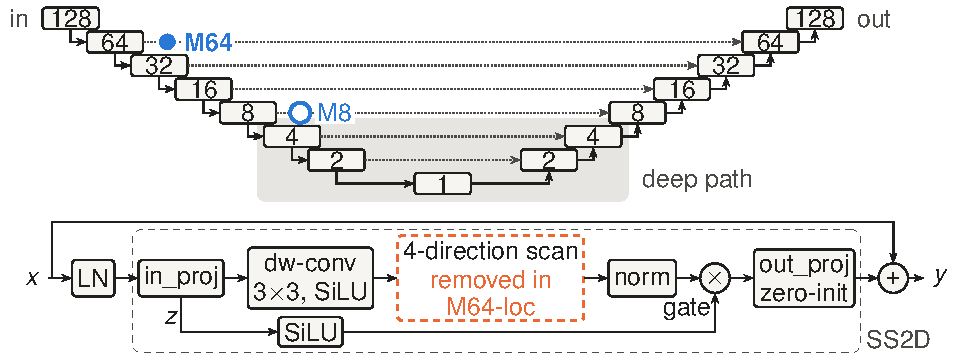
\includegraphics[width=\columnwidth]{img/fig_block.pdf}
\caption{\textbf{Top:} DfpNet with level resolutions and insertion points
(\M{64}, \M{8}; \Mdec{} sits in the decoder); the shaded deep path is pruned in
\TR{} and replaced by 11 SS2D blocks in \DR. \textbf{Bottom:} residual block
with the SS2D mixer; in \Mloc{} (M64-loc) the scan is replaced by $D\mathbf{x}$.}
\label{fig:arch}
\end{figure}

Each configuration adds one residual block,
$\mathbf{y} = \mathbf{x} + \mathrm{Mixer}(\mathrm{LN}(\mathbf{x}))$, after an
encoder layer, feeding both the subsequent layer and the skip connection
(Fig.~\ref{fig:arch}); the mixer is SS2D, self-attention or scan-free SS2D,
depending on the configuration. Zero-initializing the output projection
ensures exact identity with \B{} at initialization (for matched random seeds).
The SS2D mixer follows the official VMamba implementation, with $E=2n_c$ and
state dimension $N=16$.

Configurations \M{l} and \Mdec{} insert the block at resolution $l \times l$
in the encoder and decoder, respectively. \Msh{8} is an earlier simplification: the four scans share one complete
1-D Mamba layer (projections, gate and its own short convolution, no output
norm), and their outputs are summed. \SA{64} uses 4-head self-attention. For
deep-path analysis, \TR{} truncates DfpNet below $8\times8$, while \DR{}
replaces the pruned layers with 11 SS2D blocks, parameter-matched to B.

To isolate the scan, \Mloc{} replaces each scan path with its skip term
$D\mathbf{x}$~\eqref{eq:ssm}. This block is close to the local Gated CNN of MambaOut~\cite{yu2025mambaout}, with no spatial
propagation beyond $3\times3$. Five ablations remove one component at a time
(gating, output/input norm, expansion, or a dense convolution). As controls,
\Conv{} uses two $3\times3$ convolutions (similar parameter count, no norm or
gating), and \Blarge{} widens \B{} to 33 base channels, adding about as many
parameters as the $8\times8$ blocks without a new block. Additional variants
($32\times32$ insertion, multi-block placement) yield consistent findings.

\subsection{Protocol and statistics}
\label{sec:protocol}

All models follow the repository's training protocol: Adam optimizer
($\text{lr}=6\times10^{-4}$, $\beta=(0.5,0.999)$), L1 loss, batch size 10,
evaluation of the final checkpoint. The learning rate is constant for the
first half of training, then decays towards $0.1\,\text{lr}$; as this schedule
is defined in epochs, we fix 133 epochs (79,667 iterations), the longest of
three budgets (17, 67, 133) whose validation gain over the previous one
exceeded the seed-to-seed noise, a rule set before the runs. To account for
non-deterministic CUDA kernels, we use 8 seeds for \B{} and primary models, 5
for ablations and \DR/\TR, and 3 for the full dataset.

Comparisons use the sample-wise mean of seed-averaged differences relative to
\B, with 95\% confidence intervals (CI) from a two-level
bootstrap~\cite{efron1993}: each of 10,000 repetitions resamples the seeds of
each configuration (training variability) and the airfoils with all their
samples (flow conditions of one airfoil are correlated). A CI containing zero
indicates ``no demonstrated difference'' rather than equivalence.

Following exploratory validation, test evaluations were pre-registered (specifying hypothesis, metric  and the criterion ``confirmed if the upper bound of the 95\% CI
of the difference to \B{} is below zero'') and executed exactly once across five passes:
(1) $8\times8$/$32\times32$ blocks and \Blarge{} on \relall;
(2) \M{8};
(3) \DR{} with \TR{} as control;
(4) \M{64}; and
(5) \Mloc{} on \relvy{} (hypotheses 4--5 derived from validation, with 5 dependent on 4).
Most experiments ran locally on an RTX~4060 Laptop GPU (8\,GB), while the full dataset ($\approx$20\,GiB) used a cloud VM with an NVIDIA L4 GPU.

% =====================================================================
\section{Results and discussion}

\subsection{Mamba is redundant, yet replaces the deep path}
\label{sec:deep}

On the test set, inserting a Mamba block at $8\times8$ yields no performance
improvement (Table~\ref{tab:main}): \Msh{8} shows a \relall{} difference to
\B{} of $+0.16$ \ci{-0.10}{+0.53}, whose lower bound rules out any reduction
larger than 0.10 points (3.6\% of \B's error), while \M{8} yields $-0.01$
\ci{-0.34}{+0.26}. These blocks add capacity rather than useful
representations: on the training set, \M{8} achieves a 16\% lower L1 loss than
\B{} without improving validation L1, while \Blarge{} fails to improve
training fit.

As hypothesized (Sec.~\ref{sec:unet}), the deep path provides sufficient
global receptive field. On the 5,598-file split (Sec.~\ref{sec:data}),
truncating it (\TR) is clearly worse on validation (\relall{} $+0.73$
\ci{+0.58}{+0.89}), while on the test set the interval touches zero ($+0.57$
\ci{-0.01}{+1.03}). Replacing the pruned layers with 11 SS2D blocks (\DR)
recovers the loss (\DR$-$\TR{} $-0.69$ \ci{-1.10}{-0.26} on test) and is not
distinguishable from \B{} ($-0.12$ \ci{-0.51}{+0.29}). Hence global context is
necessary and SSM blocks can provide it, but the U-Net already captures it
(though \TR{} also removes 79\% of the parameters).

\subsection{The gain is at the highest resolution}
\label{sec:hr}

Moving Mamba blocks to higher encoder resolutions progressively improves
validation \relvy{} (Fig.~\ref{fig:abl}a), from 5.98\% at $8\times8$ to 5.32\% at $64\times64$
(baseline 6.07\%); in the decoder the block helps less. On the test set, \M{64}
confirms the pre-registered hypothesis, reducing \relvy{} by $-1.17$
\ci{-2.47}{-0.43} points (18\% relative, with 87\% of the airfoils improving)
and lowering the aggregate ratio ($-0.55$ \ci{-1.19}{-0.01}) and, almost
demonstrably, the median sample ($-0.50$ \ci{-1.25}{+0.03}), while \relall,
$\mathrm{rel}_{v_x}$ and \relp{} show no demonstrated difference. This comes at
$3.7\times$ the training time.

\subsection{Ablation: the gain does not need the SSM}
\label{sec:abl}

Fig.~\ref{fig:abl}b shows that removing the spatial scan (\Mloc) retains most
validation gains ($-0.67$ \ci{-0.98}{-0.37} vs.\ \B; $+0.08$ \ci{-0.07}{+0.25}
vs.\ \M{64}): long-range mixing is not strictly required. The gain is not
specific to Mamba: self-attention (\SA{64}) is not distinguishable from
\M{64} ($+0.13$ \ci{-0.07}{+0.35}), but requires $17\times$ the training time. Not every
block helps, though: \Conv{} shows no demonstrated gain over \B{} ($-0.12$
\ci{-0.32}{+0.07}) and is worse than \Mloc{} ($+0.54$ \ci{+0.24}{+0.89}).
Removing one component of \Mloc{} at a time never loses the gain (all variants
below \B, none distinguishable from \Mloc): the components may be partly
redundant, or the gain may come from what they share and \Conv{} lacks
(pointwise projections, SiLU, per-channel scale); our data do not separate
the two.

\begin{figure}[t]
\centering
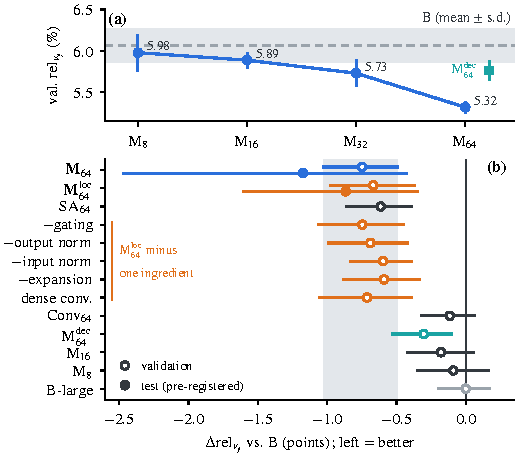
\includegraphics[width=\columnwidth]{img/fig_results.pdf}
\caption{(a) Validation \relvy{} (mean $\pm$ s.d.\ over 8, 5, 3, 8 seeds) vs.\
resolution of the encoder block; square: same block in the decoder; band: \B.
(b) $\Delta$\relvy{} vs.\ \B{} with 95\% CIs. Open: validation (8 seeds for
\M{64}, \Mloc, \M{8}, \Blarge; 5 for the others); filled: pre-registered test.
Band: validation CI of \M{64}.}
\label{fig:abl}
\end{figure}

Our final architecture combines \B{} with \Mloc{} (+7,232 parameters, +7\%
FLOPs, $1.6\times$ training time). On the test set, its pre-registered
hypothesis is confirmed: \relvy{} drops by $-0.87$ points \ci{-1.60}{-0.35}
(13\% relative), with 90\% of airfoils improving. This is about three quarters
of the gain of \M{64} ($-0.87$ vs.\ $-1.17$); the direct comparison
\Mloc$-$\M{64} ($+0.31$ \ci{-0.15}{+1.11}) shows no demonstrated difference in
either direction, so the contribution of the SSM remains undetermined. Unlike
MambaOut's dense tasks~\cite{yu2025mambaout}, spatial recurrence is not shown
to be required here.

\subsection{Expected on pressure, found on $v_y$}
\label{sec:why}

We expected gains on $p$ (Eq.~\eqref{eq:poisson}) and found them on $v_y$.
Our untested reading: the smooth, long-range part of $p$ is already captured
by the U-Net, which works like a multigrid V-cycle~\cite{he2019mgnet}, while residual $p$ errors concentrate in severe
separation tails missed by all models (2.5\% of validation samples account for
15\% of total \relp). On the test set the mean \relp{} decreases for both
blocks (\M{64} $-1.79$ \ci{-5.40}{+0.09}, \Mloc{} $-1.37$ \ci{-3.38}{-0.12}),
but for \M{64} the median sample does not move ($-0.01$ \ci{-1.43}{+0.92}): the
change sits in a few samples, and $p$ was not a pre-registered hypothesis.

The gains are instead local: within a 4-pixel wall band, the $v_y$ error drops
by 11\% (\M{64}) and 10\% (\Mloc). Since $v_y$ is mostly induced by the
airfoil, this shows in \relvy, whereas the free stream dilutes it in $v_x$ and
\relall.

\subsection{More data and limitations}
\label{sec:more}

On the full dataset (53,830 samples, including sheared airfoils; validation
only, 3 seeds, after the test passes) all models improve markedly and the gain
halves: \Mloc$-$\B{} is $-0.22$ \ci{-0.41}{-0.04} on regular validation files
($-4.7\%$ vs.\ $-8.2\%$ on the reduced set, same seeds), concentrated near the
wall (wall-band $v_y$ MAE  $-6\%$), with no demonstrated change in the aggregate ratio.

Key limitations are a test suite of 30 airfoils, five test passes, a single
optimizer for all architectures, and separated flows at high angles, which
every model misses and whose steady RANS targets may not be fully converged
(not checked).

% =====================================================================
\section{Conclusion and Future Work}

Mamba blocks bring no benefit at deep U-Net levels, where global context is
already established. At high resolution they reduce the $v_y$ error by 18\% on
the test set, a gain concentrated near the airfoil and due mostly to the local
block design: without the SSM (\Mloc) it is 13\% at $1.6\times$ the training
time, consistent with MambaOut; eight times more data halves it. Future work:
why \Conv{} fails, the share of the SSM, several scan-free blocks at high
resolution, lift and drag.

\bibliographystyle{IEEEtran}
\bibliography{references}

\end{document}